\documentclass[10pt]{article}
\usepackage[top = 0.5in, bottom = 1.0in, left = 1.0in, right = 1.0in]{geometry}
\usepackage{float}
\usepackage{amsmath}
\usepackage{graphicx}
\usepackage{indentfirst}
\graphicspath{ {../figures/} }
\title{CS 418 Final Project}
\date{December 3, 2019}
\author {Manasa Kandimalla, Shyam Patel, Carlos Antonio McNulty}
\begin{document}
\maketitle

\section*{1. Problem Selection}

For our final project, we would like to solve the problem: which personality traits (e.g., neuroticism, extraversion, openness to experience, agreeableness, conscientiousness, impulsiveness and sensation) and other factors (e.g., age, gender and education) make one susceptible to the usage of various illegal drugs. These drugs include amphetamines, amyl nitrite, benzodiazepine, cannabis, cocaine, crack, ecstasy, heroin, ketamine, legal highs, LSD, methadone, mushrooms and volatile substance abuse (VSA).


\section*{2. Data Collection}

The data for our project consists of a single dataset titled \textit{Drug consumption} donated to the UCI Machine Learning Repository in 2016. The original owners of the database are Elaine Fehrman, Vincent Egan and Evgeny M. Mirkes. The database contains records for 1,885 respondents. For each respondent, 12 attributes are known: measurements which include NEO-FFI-R (neuroticism, extraversion, openness to experience, agreeableness, and conscientiousness), BIS-11 (impulsivity), and ImpSS (sensation seeking), level of education, age, gender, country of residence and ethnicity. Each respondent also provided their usage for 18 legal and illegal drugs, including the fictitious drug Semeron. The categories for drug usage consisted of: never used, used over a decade ago, used in the last decade, used in the last year, used in the last month, used in the last week, and used in the last day.

\section*{3. Data Preparation}

The provided dataset does not include a header. For ease of use with the Pandas library, we added a header. To allow us to perform some analysis of the dataset, we needed to convert the values in the dataset to something more interpretable. For instance, the values for male and female were provided as the values -0.48246 and 0.48246, respectively. We converted these into categorial variables, at least for the duration of our analysis. We also had to label encode the drug usage responses and one-hot encode the gender category for later use with classifiers. Second, the categories of drug usage (e.g., never used, used over a decade ago, used in the last decade, used in the last year, used in the last month, used in the last week, and used in the last day) were converted into integers, after which a binary \textit{Drug User} variable was added that simply distinguishes between respondents who used any illegal drugs in the past and those who did not.

\section*{4. Data Exploration}

\begin{figure}[h]
\caption{Drug Usage}
\centering
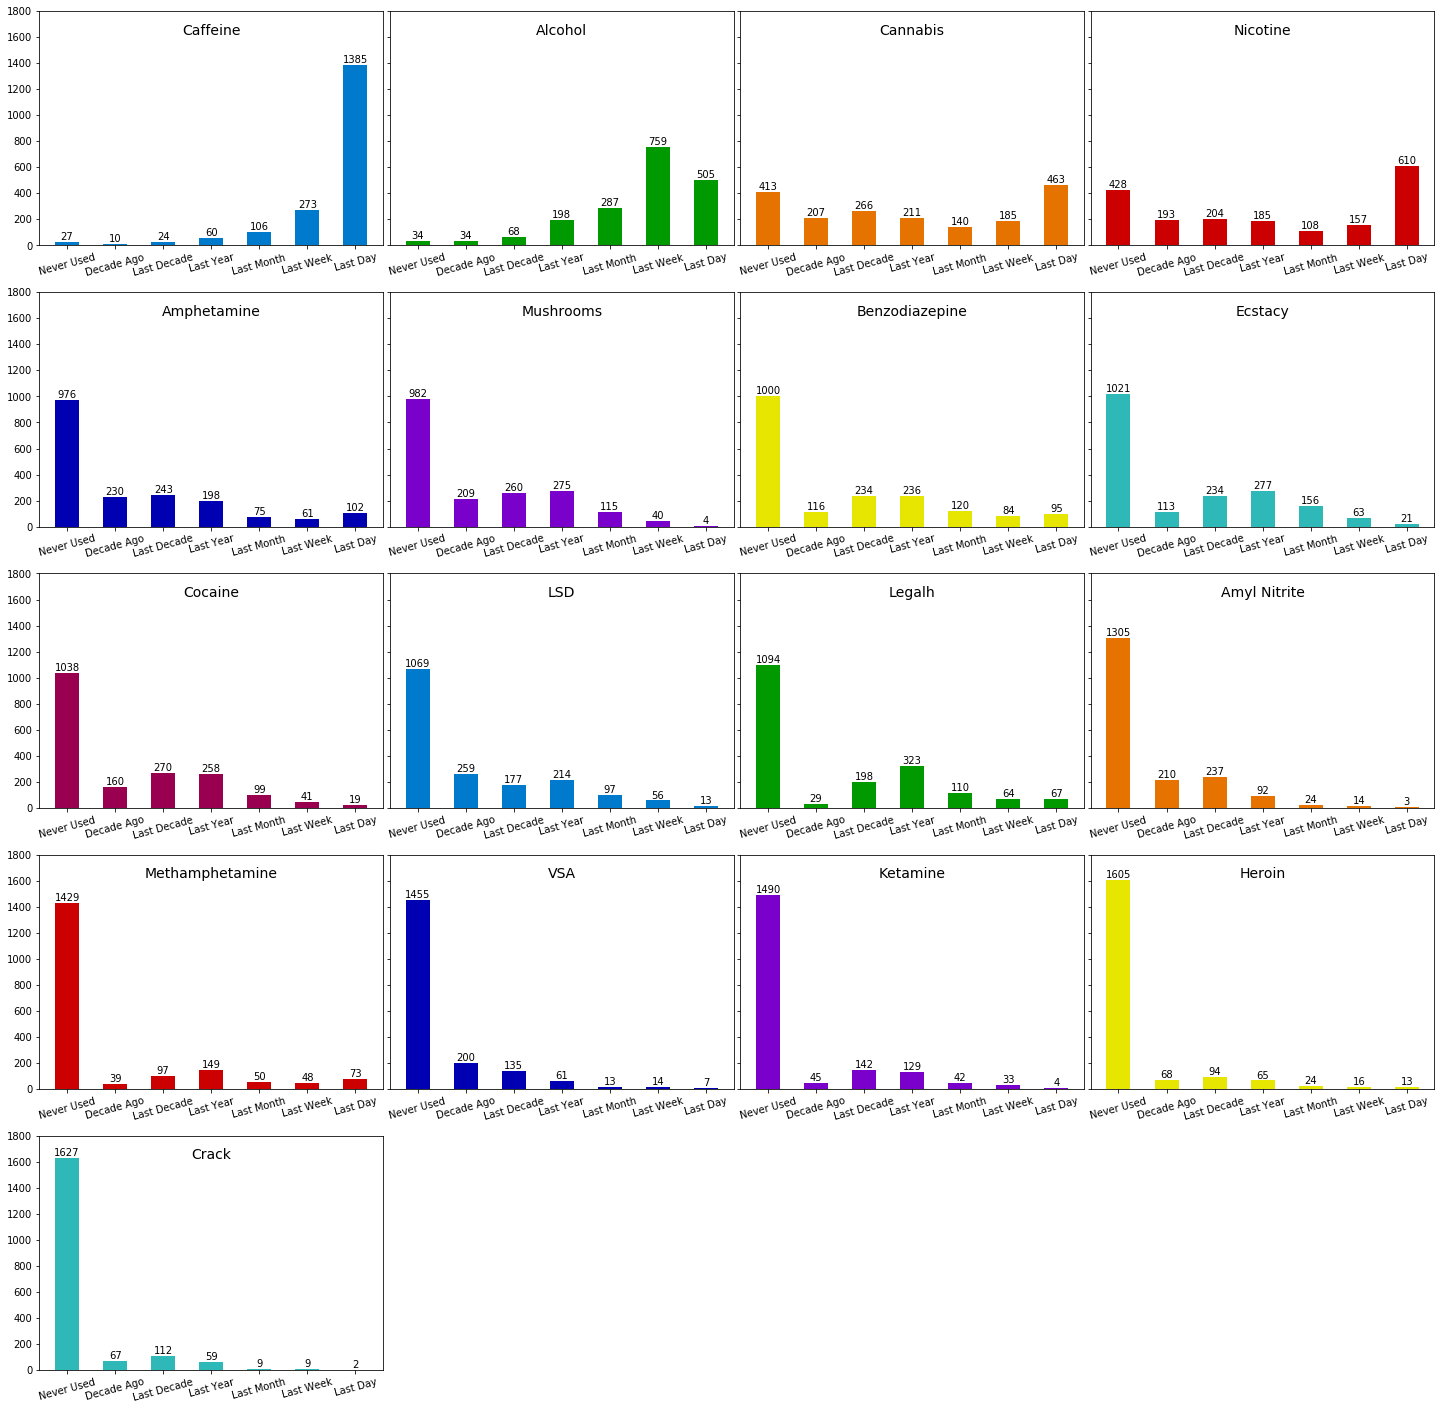
\includegraphics[scale=0.7]{drugs.png}
\end{figure}

Something...

\begin{figure}[H]
\caption{Illegal Drug Usage and Frequency by Gender}
\label{fig:genders}
\centering
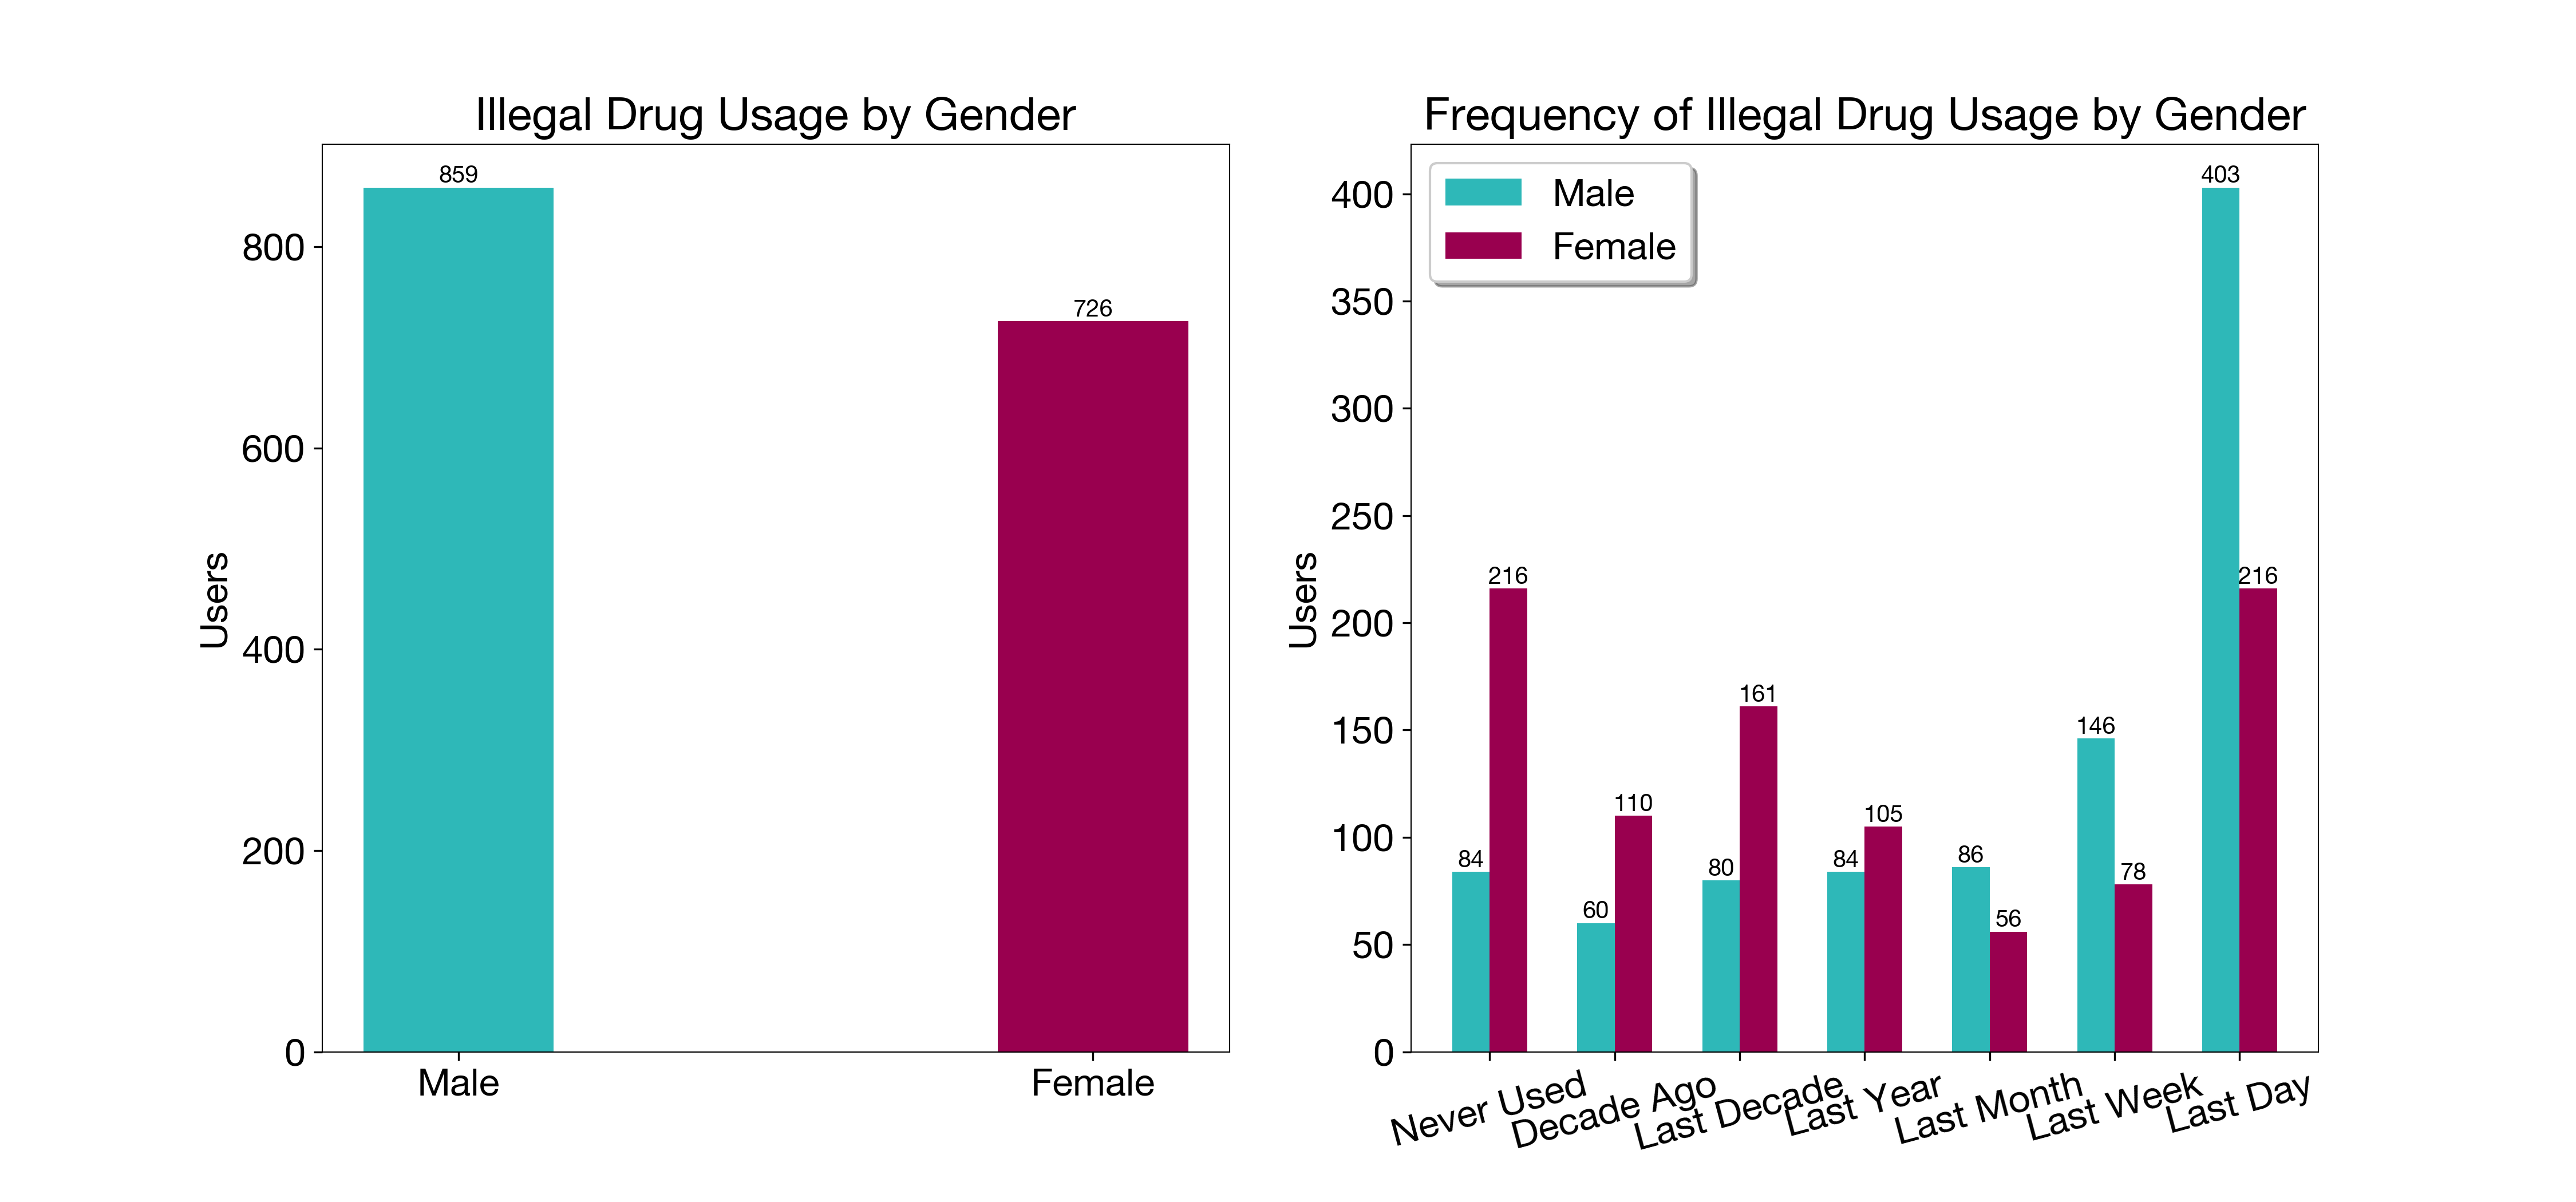
\includegraphics[scale=0.4]{gender_freq.png}
\end{figure}


\begin{figure}[H]
\caption{Illegal Drug Usage by Personality Trait}
\label{fig:traits}
\centering
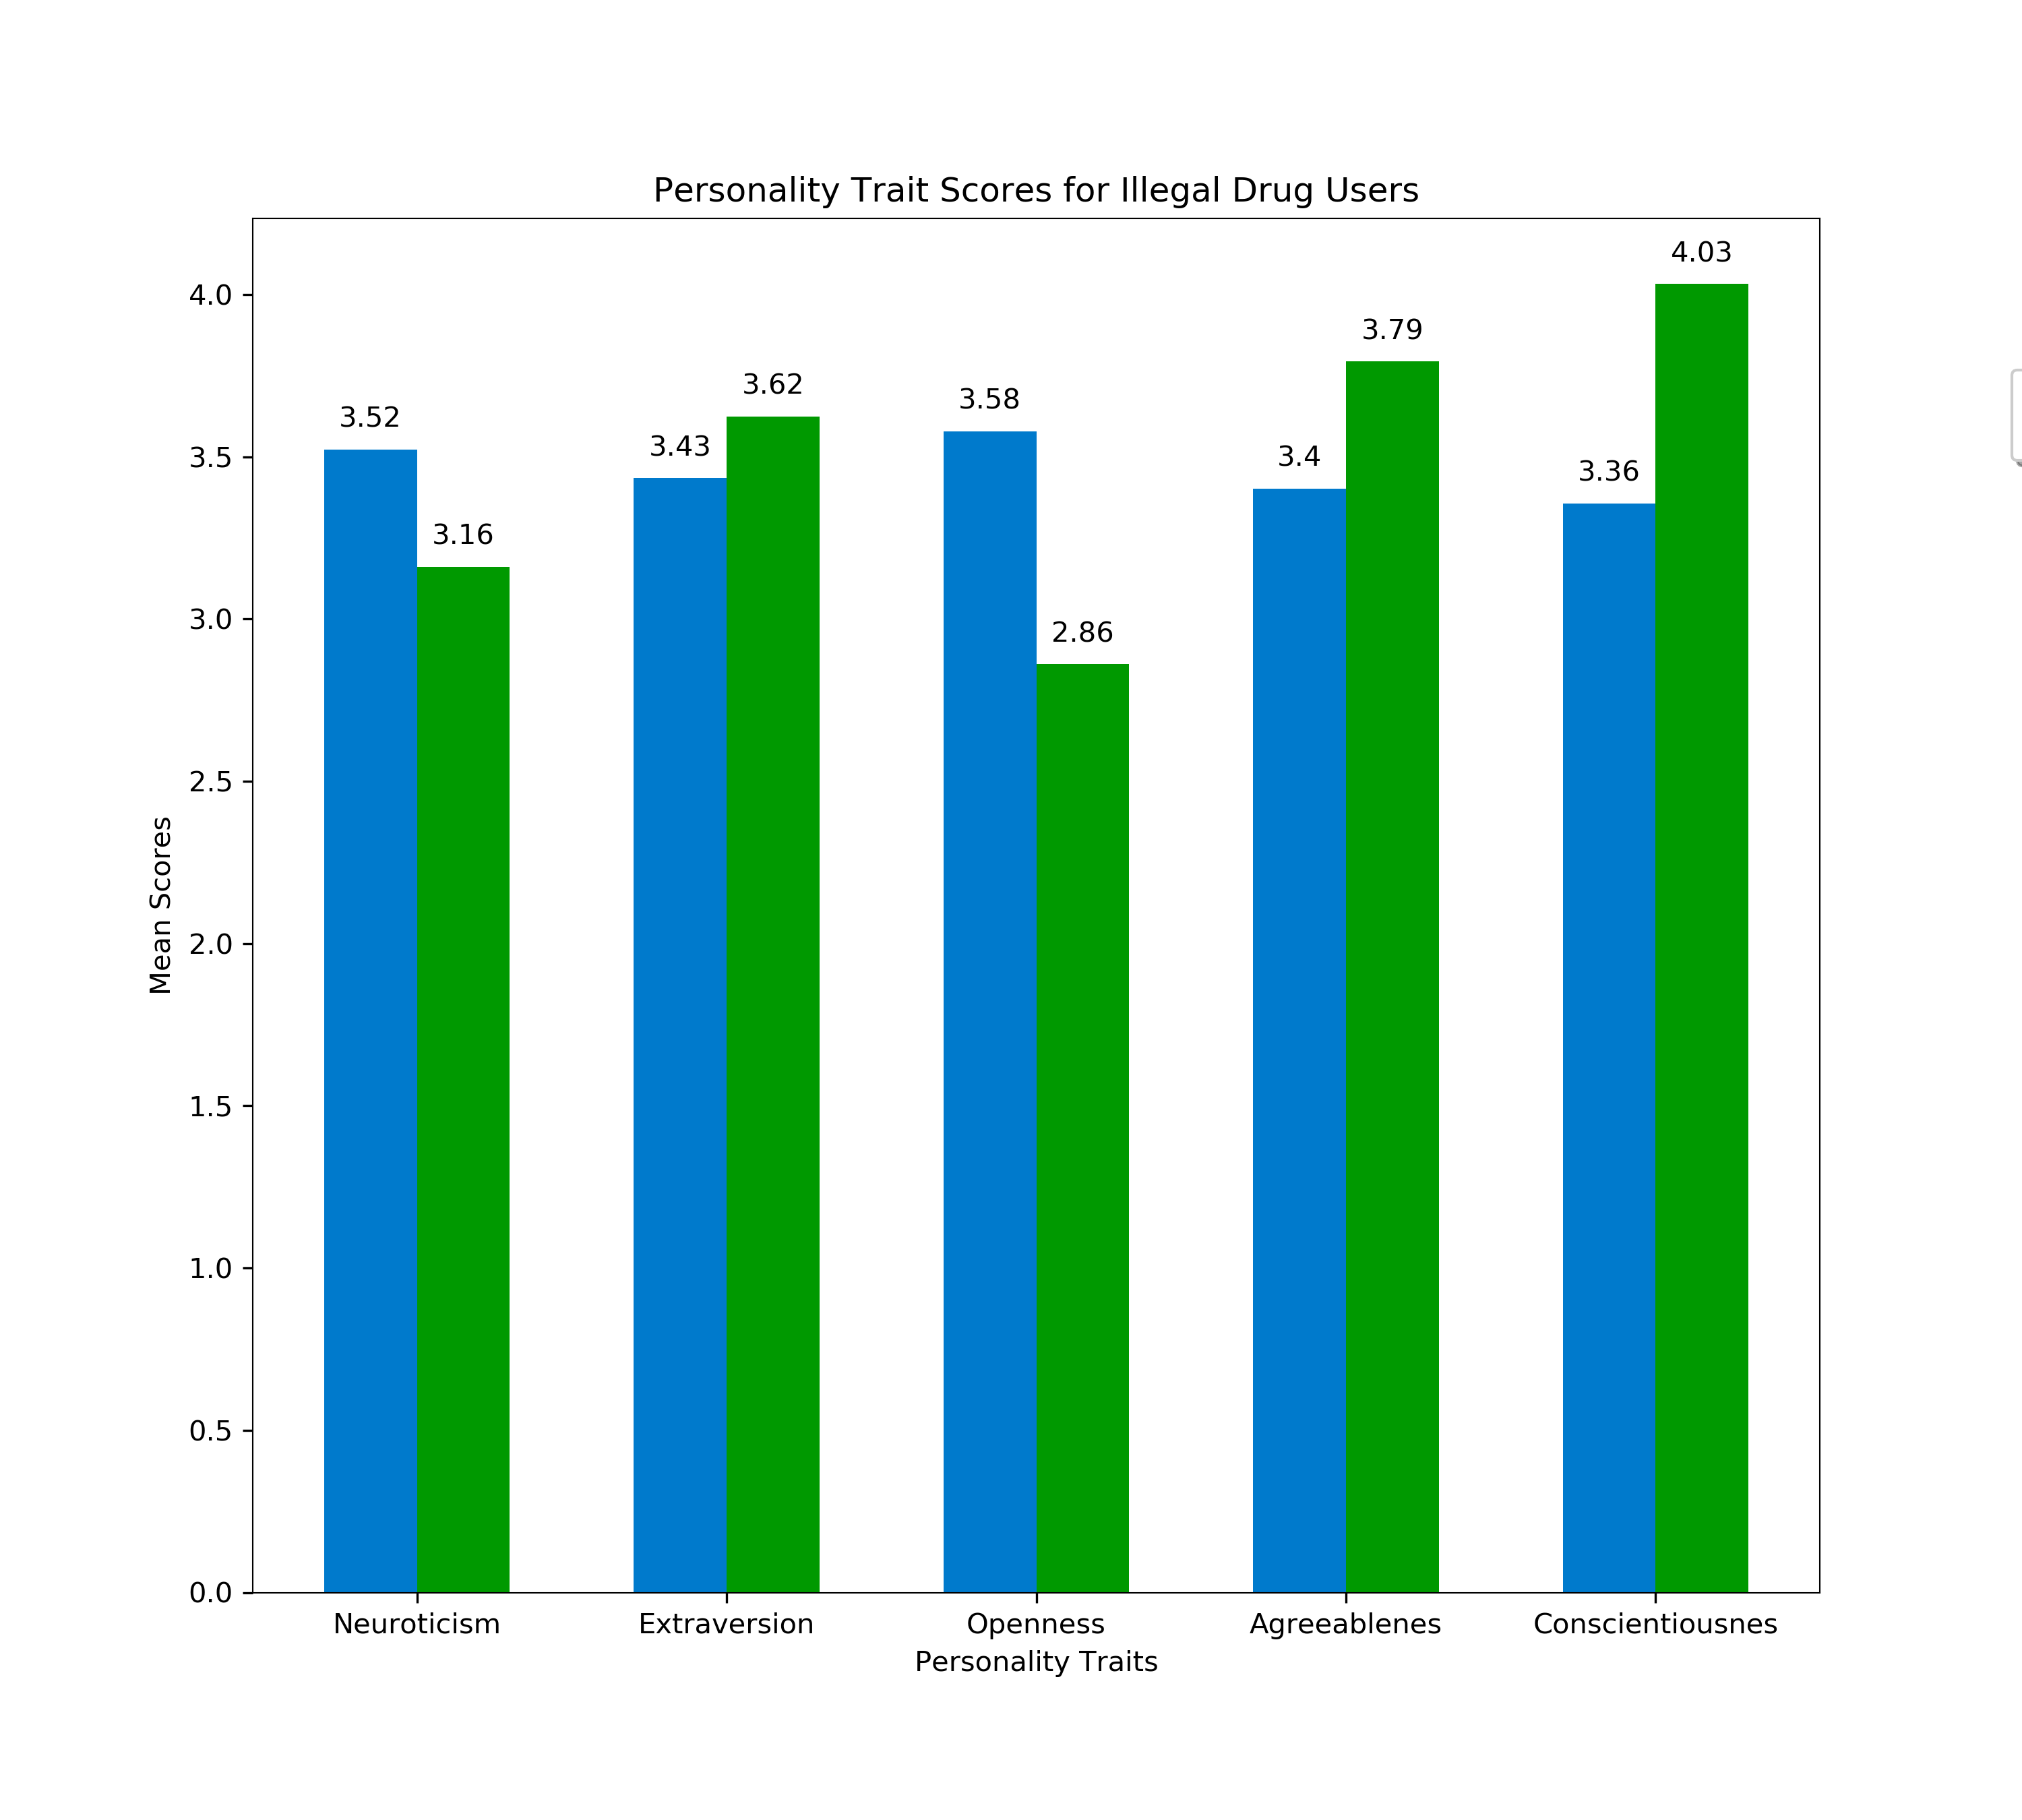
\includegraphics[scale=0.25]{traits.png}
\end{figure}

\begin{figure}[H]
\caption{Heatmap of Correlation Matrix}
\label{fig:heatmap}
\centering
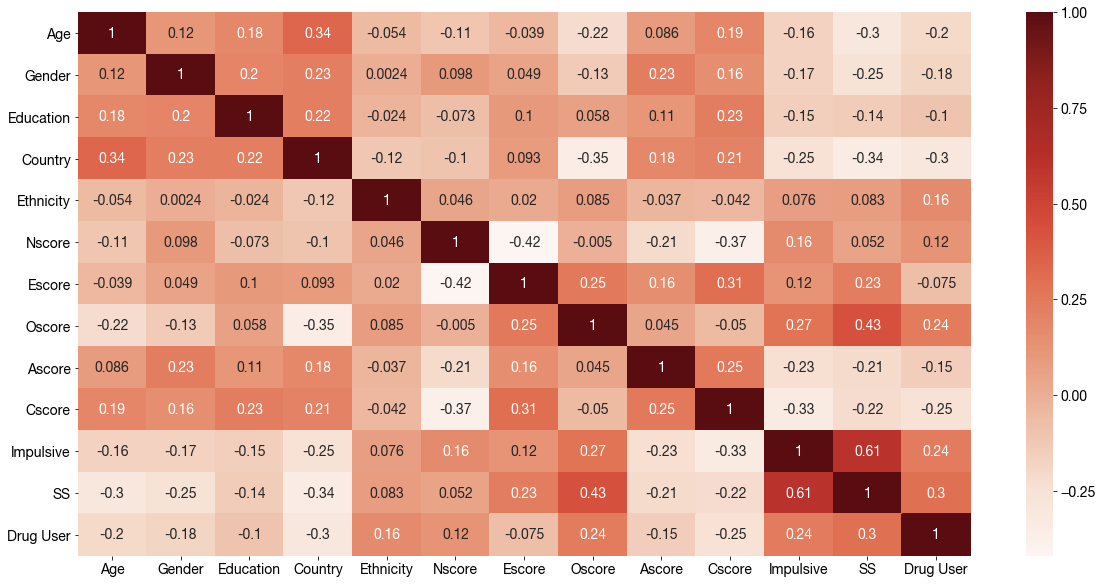
\includegraphics[scale=0.25]{heatmap.png}
\end{figure}

\section*{5. Data Modeling}

\subsection*{Decision Tree Classifier}

\subsection*{Random Forest Classifier}

\subsubsection*{Feature Selection}

To select the features for our binary classifier we consulted the pearson correlation matrix in Figure \ref{fig:heatmap}. In addition a feature selection tool from sklearn was used that determines a models features importances and removes those that fall below a certain threshold. Our analysis indicated that the features that might be best for our model were Age, Education, Country, Nscore, Escore, Oscore, Ascore, Cscore, Impulsive, and SS.

\subsubsection*{Grid Search}

\begin{figure}[H]
\caption{Hyperparameter Tuning with Grid Search }
\label{fig:gridsearch}
\centering
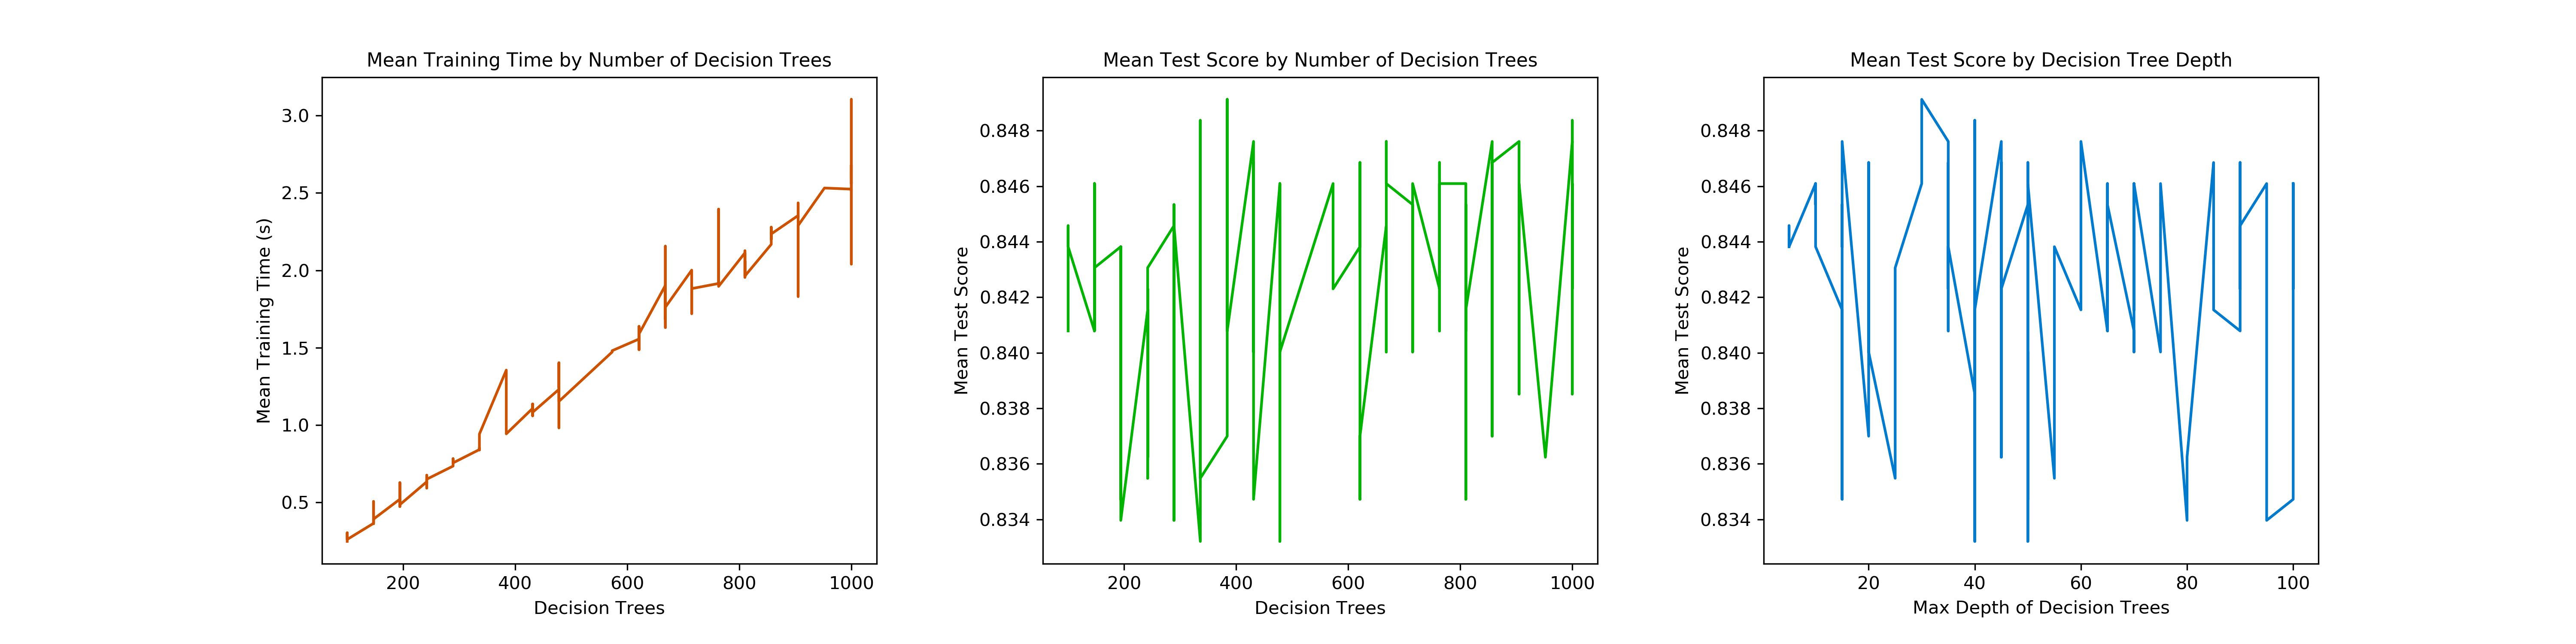
\includegraphics[scale=0.35]{gridsearch.png}
\end{figure}

We performed grid search on 30,240 random forests by varying the number of estimators and the configuration for the base estimators provided to each random forest. The exhaustive search then chose the best performing model when tested with 10-fold cross validation. This model had an F1 score of 0.844 and an accuracy of 0.913. When the model was applied to the test set it resulted in an accuracy of 0.827.

\subsection*{Clustering}

\section*{6. Results}


\end{document}